%!TEX root = ../Thesis.tex

\chapter{Workshop 1}
\label{appendix:workshop1}
\lhead{}
In de eerste workshop werd een introductie gegeven van Blueprints en \gls{ue4}.
Daarnaast werden de \"best practises\" besproken en een aantal valkuilen tijdens het modellen voor een game engine.

De workshop is opgenomen en het audio fragment is beschikbaar op aanvraag.

\section{Doel}
\begin{itemize}
	\item Het doornemen van best practises voor UE4 gefocused op verschillen tussen 3D moddeling en 3D games. 
	\item Een begin maken en kennis laten maken met Blueprints.
\end{itemize}

\section{Best practises}
De volgende problemen waren de niet-programmeurs tegenkomen en werden kort uitgelicht. Er werd ook verteld dat in tegenstelling tot het maken van statische 3D scene het maken van een 3D wereld veel fout gevoeliger is en dat er bewuster met de verschillende elementen van de engine omgegaan moet worden.

De volgende best practises werden toegelicht.
\begin{itemize}
	\item Probeer altijd de documentatie te lezen van een onderdeel voordat je het in productie wilt gebruiken.
	\item Geen scenes in Max maken maar objecten los exporteren en de scene bouwen in \gls{ue4}.
	\item Textures altijd in dimensies in de “Power of Two” maken (4, 8, 16, 32, 64, 128, 256 etc.).
	\item Texture grootte en vertices count zijn belangrijk voor performance in tegenstelling tot 3D moddeling.
	\item Maximale texture grote 4096 * 4096 (2048*2048 voor mobiel).
	\item 65,000 vertices max.
	\item Gebruik altijd het tweede UV channel.
\end{itemize}

Ook werd er gevraagd om de volgende link goed door te lezen als voorbeeld van de \gls{ue4} documentatie
\url{https://docs.unrealengine.com/latest/INT/Engine/Content/FBX/BestPractices/index.html}

\subsection{Ontwikkeling voor mobiel}
De volgende best practises met betrekking tot mobile ontwikkeling werden toegelicht:

\begin{itemize}
	\item Tijdens het opzetten van een project de target hardware setting op mobiel en de quality setting op scalable. 
	\item Het is makkelijker om de kwaliteit te upscalen dan te downscalen.
	\item Voor het mobile platform komen alle assets in de package terecht. Daarom is het belangrijk om niet gebruikte assets te verwijderen.
	\item Maximale texture van 2048*2048 en maximaal 65,000 per object.
	\item De belichting is minder geavanceerd op een mobiel. Daardoor moet er handmatig meer tijd gestopt worden in het zelf belichten van scenes.
\end{itemize}

Ook werd er gevraagd om de volgende link goed door te lezen als voorbeeld van de \gls{ue4} documentatie
\url{https://docs.unrealengine.com/latest/INT/Engine/Content/FBX/BestPractices/index.html}

\section{Workshop}
Na het bespreken van de best practises voor \gls{ue4} werd er voor gedaan hoe een lamp aan en uit gezet kan worden als de speler in de buurt komt door middel van een Blueprint. 

Er werd gevraagd of de lamp ook geleidelijk in sterkte kon toenemen en dit werd ook gedemonstreerd.

\begin{figure}[!ht]
  \centering
    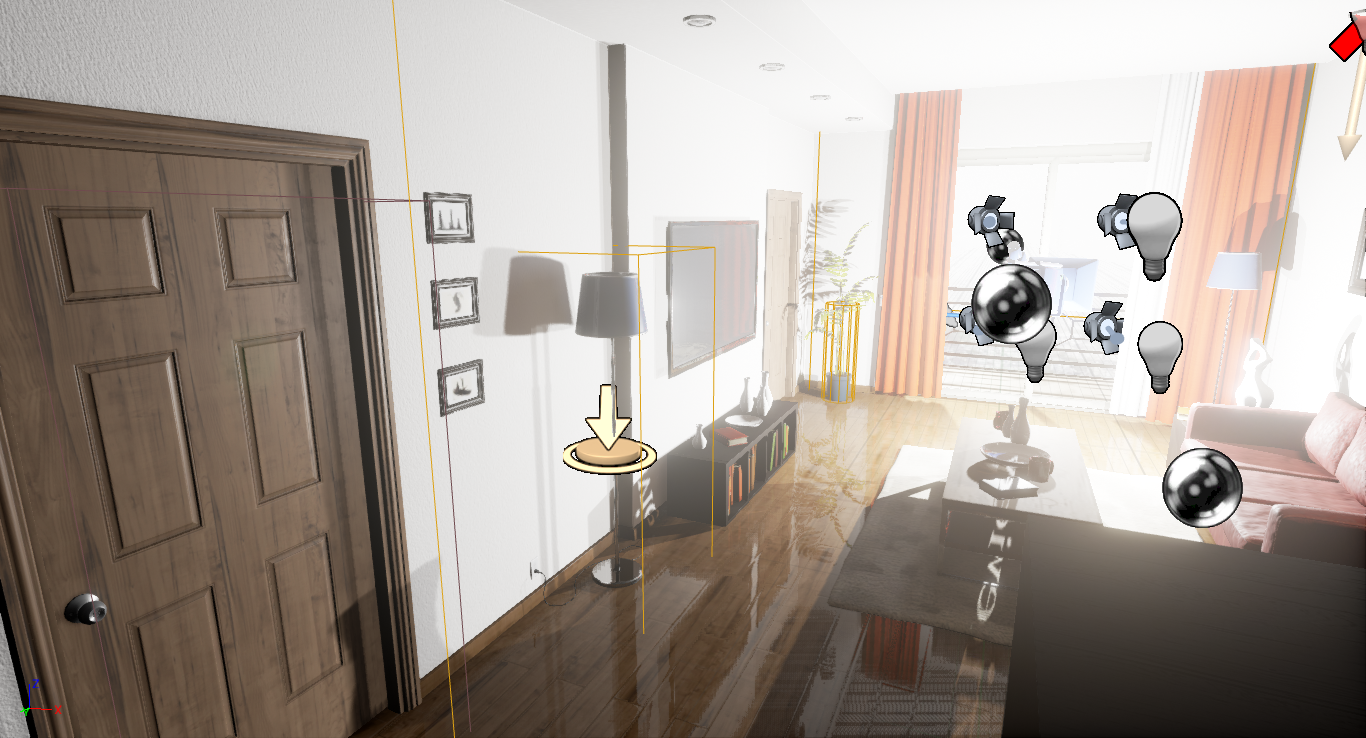
\includegraphics[width=\linewidth,height=\textheight,keepaspectratio]{Workshop_1_lamp}
    \caption{De lamp die aan en uit gezet werd.}
\end{figure}

\begin{figure}[!ht]
  \centering
    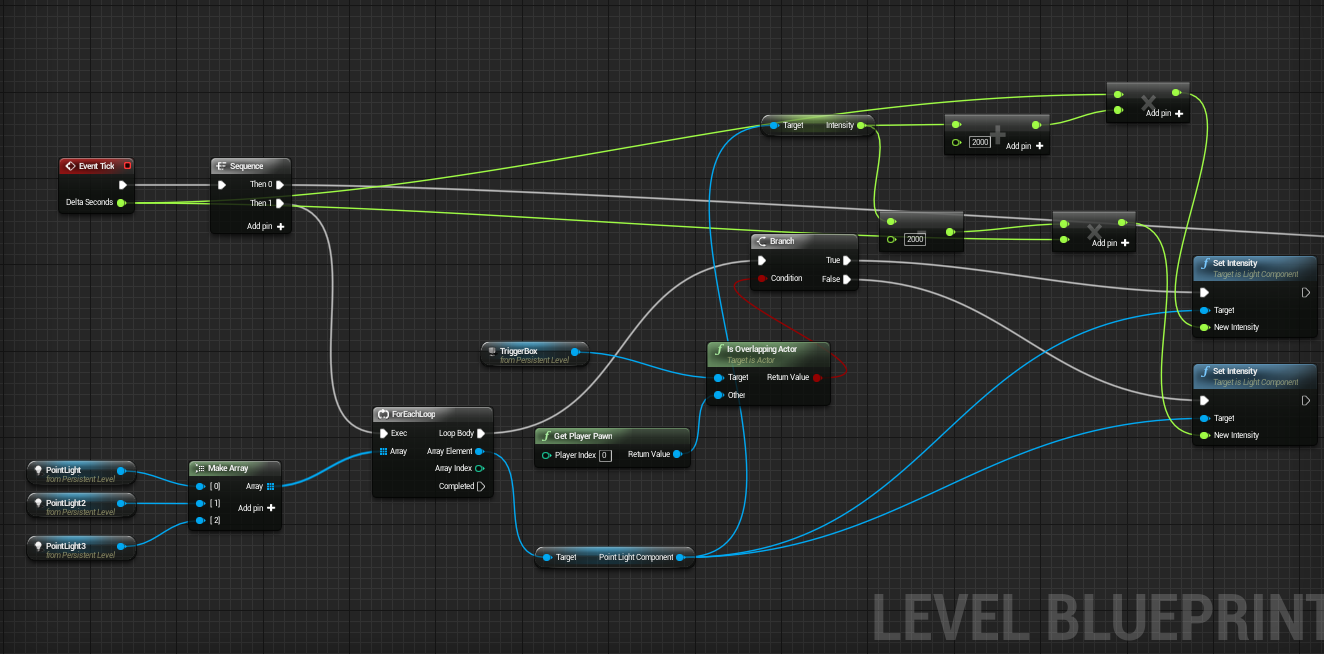
\includegraphics[width=\linewidth,height=\textheight,keepaspectratio]{Workshop_1_LampBlueprint}
    \caption{De Blueprint van het langzaam laten toenemen van de licht sterke van de lamp.}
\end{figure}

\section{Reflectie}
Na de workshop is er met de deelnemers besproken welke van de behandelde onderwerpen onduidelijk waren of interessant om dieper op in te gaan. Op basis hiervan is besloten om dieper op Blueprints, en algemene programmeer logica, in te gaan. Ook is er besloten om in de volgende workshop zelfstandig een opdracht te maken omdat vooral de onderwerpen die het best geleerd kunnen worden door middel van ervaring onduidelijk waren.